\chapter{FlipIt with propagation delay}
\label{chapter2:FlipIt with virus propagation}
%\documentclass[10pt]{article}
%\begin{document}

%%%%%%%%%%%%%%%%%%%%%%%%%%%%%%%%%%%%%%%%%%%%%%%%%%%%%%%%%%
%%%%%			Introduction Chapter 1				%%%%%%
%%%%%												%%%%%%
%%%%%												%%%%%%
%%%%%%%%%%%%%%%%%%%%%%%%%%%%%%%%%%%%%%%%%%%%%%%%%%%%%%%%%%

\section{Introduction}
\label{Ch2:Intro}
The FlipIt game with propagation delay considers a game where the moves of the attacker are not instantaneous. This corresponds to APT's which use malware - viruses, worms or trojan horses - to perform attacks, as the malware needs time to propagate. A virus, for example, can be dropped on a network but it only compromises the whole network if every node in the network is infected. So there is a certain delay between the moment of attack and the moment the attacker has control over the resource, called the propagation delay. The basic FlipIt game does not take this propagation delay into account. This chapter explains how the FlipIt game with propagation delay can be modelled. Section \ref{ch2:diffFlip} explains the difference between a basic FlipIt game and a FlipIt game with propagation delay. The last section \ref{ch2:periodicvirus} derives a formula to calculate the benefit for a FlipIt game with propagation delay. In the next Chapter, this benefit formula will be used to determine what the best defence and attack strategies are.
%Section \todo{nash} presents the Nash equilibrium for the benefit formula. The chapter concludes in section \todo{section toevoegen} with lessons learned en practical implications for cyber security.
%
%\section{FlipIt game with virus propagation}
%
%Welke aanpassing en motivatie: attacker 1 speler die elke keer virus probeert te droppen. Defender die elke keer patcht als er virus gedropt wordt. Elke patch voldoet aan de meest recente patch dus alle virussen die ook gedropt zijn worden weggedaan. Voor future work: patch systeem aanpassen. 
%
%The actions of a defender: the actions of an attacker:

\section{Difference between FlipIt with and without propagation delay}
\label{ch2:diffFlip}

%\textbf{Section:Required adaptations to the FlipIt game}

The following paragraphs will list the required adaptations to model the basic FlipIt game with propagation delay.

\subsection{Single resource}
The basic FlipIt game consists of a single resource. To represent the security problem of the propagation of an APT in a network, the adapted game defines its single resource as a computer network with multiple
nodes. One of the players, the defender, will try to defend his network.
% The defender will do this by flipping all the nodes of the network (i.e. the entire resource) in every move he plays. 
The defender will do this by flipping the nodes of the network.
The attacker on the other hand will try to infect all the nodes in the network. 
%For an attacker on the other hand, it is quite impossible to infect all computers in a network at once. Rather, t
%The attacker will try to identify the node in the graph that can infect all the nodes in the shortest possible time. Then, after dropping a virus on this first node, it takes a while for the virus to infect the entire network. \\
The attacker will do this by dropping a virus on a node on the network. The virus will then spread itself and infect other nodes in the network. \\
By defining the resource as a network with multiple nodes it is possible to increase the number of possible actions by the defender or attacker. These actions will be explained in the following subsection.
%Since the original FlipIt game works with a single resource that is always flipped entirely, the assumption is made that the attacker is considered to gain immediate full control over the resource when the network has been infected, even it is only one node that has been infected.\\
\subsection{Actions of the players}


The network is composed of multiple nodes. The defender can choose to flip one node, a subset of nodes or all nodes of the network. In this paper, the defender flips all the nodes in the network every time he plays. This action can be extended to flipping only a subset of the nodes or a single node of the network. This extension has already been investigated in the context of placing anti-virus systems in a graph. This problem is known to be NP-hard. \cite{NPhard}. \\ \todo{niet volledig juist, defender systemen geplaatst en dan gezien hoe ver de worm kan geraken}
The attacker only has one action: sending different kinds of malware to a computer network. Every time the attacker flips the resource, he does this by sending a new kind of malware e.g worm to the system. The attacker does not send the same malware again, because if the computers are patched, the malware will be unable to penetrate the system. The node can be a targeted node or a random node. If the attacker has knowledge about the topology of the network, the attacker can choose to target a specific node. Most likely, this will be the node that can infect all other nodes in a minimum timespan.
\subsection{Immediate effect of the move}
%The framework of FlipIt is used to model targeted attacks. In FlipIt when an attacker attacks, he will get immediately control over the resource. One of the differences is that FlipIt does not consider that moves of the attacker might not be instantaneous. 
%With FlipIt with a propagation delay we model the fact that if the attacker flips, he does not get immediate control over the resource.  This is motivated by the fact that it takes a while before a targeted attack can compromise a computer network. The virus or worm has to spread to infect sufficient computer controlled device in the network. This propagation make take a while. \\
%In reality however, after dropping a virus on the first node, it takes a while for the virus to infect
%the entire network. So, the assumption that the attacker has full control over the resource as soon as a node has been infected, is not realistic. The attacker has only control of the network once all or a sufficient number of nodes are infected. 
The time that it takes for a piece of malware to infect every node (or a sufficient number of nodes) will be
denoted as a propagation delay variable \textit{d} (called 'delay' for short in the remainder of this paper). If we want to measure how long it takes for the malware to infect all the nodes in the network, we have to calculate the shortest path from the
first infected node to the farthest node. Rather than denoting the time needed for infecting \textit{all} the nodes, the variable $d$ can also be used to denote the time needed to infect \textit{a sufficient number} of nodes. \\
The moves of the defender are immediate. It is assumed that if a defender tries to clean the network that this will happen without a delay. The defender can de-plug the computer from the network, push a security update to all pc's, or even format a pc. 
\subsection{Stealth character of the move}
Moves in the basic FlipIt game are stealthy or covert and not immediately detected by the other player. The attacker's moves are stealthy because we want to model a scenario where a computer network is attacked by an APT. The main characteristic of an APT is that the attack is stealthy. Depending on how the attacker has set up his attack, and depending on whether or not the network is connected with the Internet, the moves of the defender are stealthy or not stealthy. For example, if the attacker launches an APT only to harm the system and not to receive feedback, the moves of the defender are stealthy. If the attacker launches an APT to steal sensitive information, the moves of the defender are non stealthy because if the defender takes actions the attacker can see that he does not receive information any more. \\
In this paper we assume that both moves of the attacker and the defender are stealthy. Our motivation for a defender with stealthy moves is that it can not be assumed that every attacker can receive feedback from an APT. Some APT's can be resident on a isolated network (e.g. Stuxnetworm), meaning that there is no way to connect to the internet. \\
%Another example is by the use of honeypots. 
Even when the APT is launched to steal sensitive information the defender can set-up a honey pot, making the attacker believe that he is stealing sensitive information, but the information in the honeypot is all fake. Honeypots emulate services or creates multiple instances of real operating systems and can pretend to have sensitive information.  Honeypots do not detect all malicious attacks so the attacker can stay unnoticed and can still provide information as feedback. Furthermore, the case where the moves of the defender are non stealthy has already been investigated by Laszka \citep{MitigationNonTargeted}.


  
\subsection{Cost associated with the move}
 The defender will defend every computer-controlled device in a network. In order to clean the network, the defender can patch the systems with the latest security bulletins, reinstall the software or even format the computer. All these different actions can imply other costs. The cost of patching a system, for example, will most likely be smaller than replacing a computer. \\ 
The cost of the attacker depends on the complexity of the vulnerabilities exploited and how difficult it was to program the malware.
\subsection{Strategies}
The formal definition of the adapted FlipIt game starts from the model of the non-adaptive continuous basic FlipIt game where players use a periodic strategy with a random phase. \\

\textbf{No feedback (non-adaptive)}\\
Non-adaptive strategies are chosen because of the assumption that both players will receive no feedback during the game. This is motivated by the fact that the identity of the attackers and their attack strategy is rarely known to the defenders. In the case of the attacker, if an attacker wants to have feedback it may be disadvantageous if he wants to stay undetected. If the attacker wants to have feedback, the malware needs to make a connection with the attacker to provide this feedback. For example, this can cause more network traffic for the defender to detect. \\

\textbf{Periodic strategy}\\
The choice of periodic strategy is motivated by the assumption that in most organisations, the defence strategy is to periodically defend the network.  This is true for the example of patching. Companies like Microsoft and Google release their security patches at fixed intervals, so companies will apply these patches as they come out. Microsoft security bulletins are released on the Second Tuesday of each month. \cite{MicroPatch} \\

In the basic FlipIt game \citep{FlipIt} the authors van Dijk et al. concluded that a periodic strategy is the dominant strategy against all other renewal strategies if the opponent uses a periodic or non-arithmetic renewal strategy.  So regardless of whether the defender chooses to play periodically or not, it's a good choice for the attacker to play periodically as well. \\

The paper from Laszka \citep{MitigationNonTargeted}, which is similar to this one, also concluded that a periodic strategy is the dominant strategy against all other non-adaptive strategies.
%This corresponds to a periodic defender strategy.   %, as this also corresponds to a common real life strategy. %nog eventueel verder te motiveren
Further research can investigate the effect of relaxing this assumption. \\

%---Periodic is probably the strategy most widely used in practice as most systems require passwords, cryptographic
%keys, etc. to be changed at regular intervals, for example, every thirty days or every three months.
%In [13], it was shown that the periodic strategy strongly dominates all other renewal strategies if the other
%player uses a periodic or non-arithmetic renewal strategy. Thus, the periodic strategy is a good choice for
%an attacker who plays against a non-adaptive (NA) defender.---








%\subsubsection{Real world example: Wormlike ATP}
%Businesses are under constant attack of different threats. If an APT manages to successfully enters a companies network can cause a lot of damage. In this example the ATP will be an attacker that sends worms with stealthy features to attack a company network. He will keep on doing this, which is the persistent thing of the APT. The defender is unaware that an APT is infecting his company network. It is better for a company to assume that it is under attack. \\
%The worm can use the computers on the network as botnets or steal sensitive data. By patching or installing new software the worm can be removed form the systems. The important assets of the defender to secure in a company network are the computers, servers, data, files, and so fort. In this particular example the resource to defend consists of all the computer controlled devices on the network, e.g. servers and computers. The attacker can drop the worm through a USB stick or by tricking a victim to open or download a malicious program. The last one can be achieved by a trojan horse. 
%%------------------------------------------------%
%%            Intro Game Theory 					 %
%%------------------------------------------------%
%\subsection{Actions of the attacker}
%A virus has different kind of ways of making his way through a company network. We will describe the different ways of how the virus can propagate. For start we will say that the virus or worm will be dropped on Node i and that it has k numbers of neighbours. 
%\begin{enumerate}
%\item Node i is infected and will spread the virus or worm to every k neighbours and will stop infecting the neighbours in the next step
%\item Node i is infected and will spread the virus or worm to every k neighbours and will keep on spreading the virus to the same neighbours in every next step
%\item Node i is infected and will spread the virus to only one of the k neighbours and will stop infecting another neighbour in the next step
%\item Node i is infected and will spread the virus to only one of the k neighbours and in the next step it will infect another one of the k neighbours 
%\end{enumerate}
%
%In the game that will be modelled in the paper we will use the settings of the first spreading method. We will not use method 2 because this kind of propagation will float the network. Because we use the settings of a mail system and contact in a mailing list the method of 3 and 4 are not used. \\
%In the first method the node that has been infected can be again infected. If one of the neighbours infects the node again the node will infect his neighbours again. By using this spreading method we have three distinct states in which a node can be situated. An \textit{infected state}, a \textit{clean state} and a \textit{spreading state}. An infected state means that the node is infected and will not spread the virus to its neighbours, a clean state means that the node is not infected on that moment and a spreading state means that the node is infected and that it will spread the virus or worm to its neighbours in the next step.
%We can argument this kind of propagation through a mail worm. \todo{voorbeeld geven van zo een worm}
%%Another propagation method is that the virus works as a token. It will propagate to only one neighbour and continue to spread. 
%
%The Attacker itself has two different ways of attacking the company network. It will only infected one node of the network and will wait for the virus to spread itself through the network. We will model two ways of attacks of an Attacker:
%\begin{enumerate}
%\item The attacker drops the virus on a random node on the network
%\item The attacker drops the virus on a targeted node on the network
%\end{enumerate}
%The attacker in this game will put a virus or worm on one of the nodes in the network. (This will happen at random.) The attacker does not know on which node the virus will be dropped. We will use this randomness because \todo{feit uit security rapport symantec} most viruses are spread via a usb stick or a shared resource. If we use this spreading method where we have a targeted attack the attacker will have more information about the network. \\
%
%The attacker can choose at which rate it will drop a virus on one of the nodes on the network. The cost of dropping a virus will be the same. It will not increase. If it will increase this means that the attacker will eventually drop out of the game because it becomes to expensive.\\
%The attacker is in control over the game if it manages to infect a subset of all the resources of the company network.
%
%
%\subsection{Actions of the defender}
%The attacker wants to protect all the nodes of his network. It can do so by getting back control over the resources. We will assume that the defender of the network has knowledge over his own network. Which is convenient in the real world because a company has to know how his infrastructure looks like.\\
%
%The defender has two possible ways of defending its network:
%\begin{enumerate}
%\item The defender flips all the nodes of his network
%\item The defender will flip a subset of the nodes of his network
%\end{enumerate}
%
%The cost of flipping all the nods of the network will be greater than the cost of flipping a subset of nodes. We make this assumption because otherwise it will be beneficial for the defender to always flip all the nodes in the network.\\
%
%We will also make the assumption that as a defender flips a node the node can get infected again. A flip will not be  correlated to a patch but to a clean-up. \todo{waarom geen patch, wormen kunnen veranderen gaandeweg}
%\todo{andere mogelijkheid:} Another setting of the game can be that the flip of the defender is equal to a patch and that the resource cannot be infected any more. But with this case we deviate from the flipIt game, because the attacker cannot flip the resource any more. Unless we work with different virusses every time the attacker flips. We start with the less complex game of flipping is equal to a clean-up.




\section{Formalization of the periodic game with propagation delay}
\label{ch2:periodicvirus}

 A Periodic strategy is a non-adaptive renewal strategy where the time intervals between consecutive moves are a fixed period, denoted by $\delta$. It has a random phase, that is chosen uniformly and randomly in the interval $[0,\delta]$ for the first move. The average rate of play of a player is denoted by $\alpha_{i} = \dfrac{1}{\delta_{i}}$. Given below is a list of symbols that will be used throughout the paper. Figure \ref{FlipItDelay} clarifies the main symbols.\\
~~\\

\begin{figure}[hbtp]
\centering
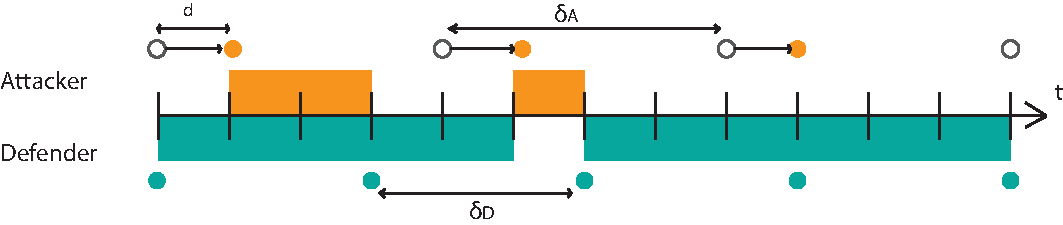
\includegraphics[scale=0.7]{Images/DefFlip.pdf}
\caption{Formalization of a FlipIt game with delay: A representation of a FlipIt game where both players are playing periodically. Every move or flip is indicated by a green or orange circle, respectively dark gray and light grey.  The defender is represented in blue (dark grey) and plays with a period of $\delta_{D}$. The flip of the attacker is represented by a white circle, but because there is a delay d, the attacker only controls the resource after time d represented by an orange circle (light grey). The attacker plays with a period of $\delta_{A}$. The green and orange rectangles represent the amount of time the respective player is in control of the resource.}
\label{FlipItDelay}
\end{figure}

\begin{description}
\item $i$: Denotes the player. \textit{D} denotes the defender, and \textit{A} denotes the attacker which differs form the notation in \citep{FlipIt}, where the defender is denoted by the subscript \textit{0} and the attacker by the subscript \textit{1}.
\item $\delta_{i}$: The length of the interval between two consecutive moves of player \textit{i}. 
\item $\alpha_{i}$: The average flip rate of player \textit{i}, given by $\alpha_{i}=1/\delta_{i}$.
\item $k_{i}$: The cost of player \textit{i}'s moves.
\item $d$: The delay caused by the virus propagation.
\item $G_{i}(t)$: The total gain of player \textit{i}, which is the amount of time player \textit{i} is in control over the resource up to time \textit{t}.
\item $\gamma_{i}$: The average gain rate of player \textit{i}, defined as $G_{i}(t)/t$
\item $\beta_{i}$:  The average benefit rate up to time \textit{t}, defined as  $\beta_{i} = \gamma_{i} -k_{i} \alpha_{i} $.
\item $opt_{i}$: The optimum function for player \textit{i}. 
\end{description}

The adaptation of the FlipIt model starts from the assumption that, when an attacker attacks at time \textit{t}, he doesn't get immediate control over the resource, but he only gains control at time \textit{t + d}, with $d$ denoting the time needed to infect a sufficient number of (or all) nodes. If the defender flips the network before the period $d$ has elapsed (so, somewhere between $t$ and $t + d$), then the attacker will never gain full control over the resource. (See figure \ref{dt} at point 3 and 4). This implies that the mathematical formulas for gain and benefit need to be adapted to the fact that the attacker loses part of his benefit because of this delay. In the remainder of this paper, we will adapt the formalization of the FlipIt game using the delay variable $d$. \\ 

\begin{figure}[hbtp]
\centering
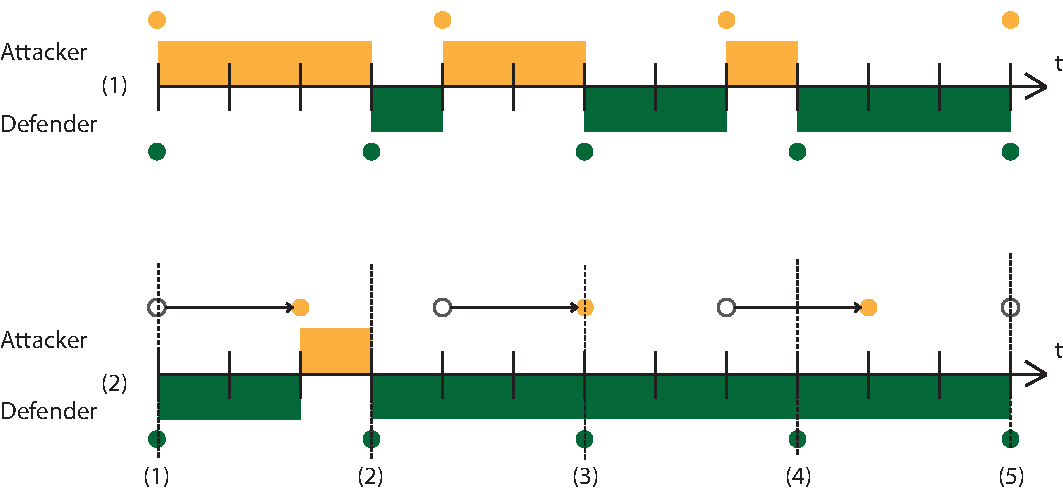
\includegraphics[scale=0.7]{Images/Delayuitgelegd.pdf}
\caption{The first game is the basic FlipIt game. The second is the FlipIt game with a delay. During the first flip of the attacker, the defender moves after the delay, causing the attacker to get control over the resource. During the second flip of the attacker, the defender flips at time t+d, causing the defender to take control over the resource before the attacker. During the third and final flip of the attacker, the defender flips during time t+d, causing the attacker to never gain control over the resource. }
\label{dt}
\end{figure}

Similarly as in \cite{FlipIt}, we split the formalization in two cases. In the first case the defender plays at least as fast as the attacker, in the second case the attacker plays at least as fast as the defender. For each of these cases, the benefit formula of the basic case without delay is presented first, and subsequently the delay is introduced.  \\

Intuitively, we could assume that $d$ can never be bigger than $\delta_{A}$ because then the attacker would play again before the delay has finished. This would seemingly result in a gain for the defender that is always 1, but this is not always true. Assume for example that an attacker plays with an interval of 3 time units, that the delay is equal to 4 time units and that the defender only plays every 8 time units. This situation is represented in figure \ref{langedelay}. Since the delay is shorter than the period of the defender, the attacker takes control of the resource once the delay has elapsed, until the defender plays. However, if the delay is larger that the period of the defender, then the defender will always be in control. This situation is represented in figure \ref{langeredelay}, where the attacker plays with an interval of 5 time units, the delay is equal to 6 time units and the defender plays with an interval of 4 time units. From this we can conclude that it only makes sense to calculate the formulas for the cases where $d$ is smaller than $\delta_{D}$. We can already conclude that it is of no use for the attacker to play when the delay is bigger than $\delta_{D}$. 




\begin{figure}[hbtp]
\centering
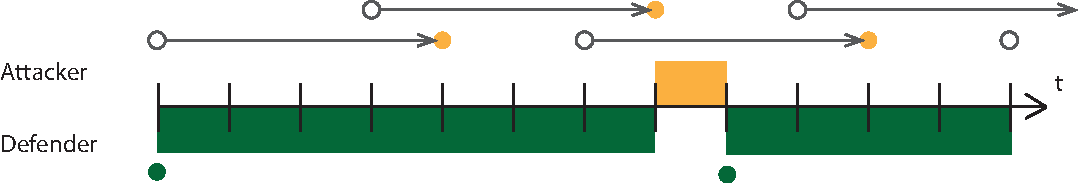
\includegraphics[scale=0.7]{Images/FlipItCase1delay.pdf} 
\caption{FlipIt with delay propagation where $\delta_{D} > d > \delta_{A}$.   }
\label{langedelay}
\end{figure}

\begin{figure}[hbtp]
\centering
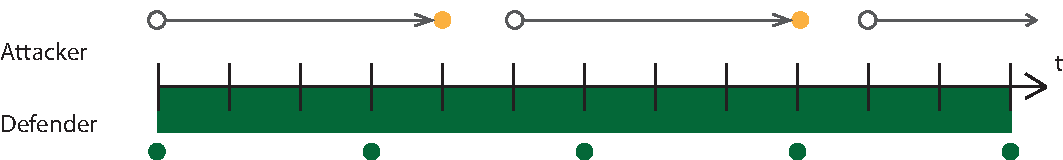
\includegraphics[scale=0.7]{Images/FlipItCase1delaytobig.pdf} 
\caption{FlipIt with delay propagation where $ d > \delta_{D}$ }
\label{langeredelay}
\end{figure}


In the original model of FlipIt \cite{FlipIt}, the authors express the formulas in terms of $\alpha_{D}$ and $\alpha_{A}$. However, when introducing the delay, some formulas become much simpler when expressed in terms of $\delta_{D}$ and $\delta_{A}$. Therefore in the remainder of this paper, we will formulate the model using both $\alpha_{i}$ and $\delta_{i}$, depending on which variable gives the simplest representation of the formulas.

\subsection*{\textbf{Case 1:} $\delta_{D} \leq \delta_{A} $ (The defender plays at least as fast as the attacker.) }

Let $r = \dfrac{\delta_{D}}{ \delta_{A} }$. The intervals between two consecutive defender's moves have length $\delta_{D}$. Consider a given defender move interval. The probability over the attacker's phase selection that the attacker moves in this interval is r. Given that the attacker moves within the interval, he moves exactly once within the interval (since $\delta_{D} \leq \delta_{A} $) and his move is distributed uniformly at random within this interval. \\

The expected period of attacker control within the interval as the moment on which the attacker gains control is uniformly distributed over the defender's interval. On average the attacker will gain control at time r/2. So the expected gain is equal to the remainder of the defender interval, i.e. r/2, without considering the delay by a virus. Therefore the benefit for the attacker, without considering the delay, can be expressed as follows:

\begin{equation*}
\beta_{A}(\delta_{D},\delta_{A}) =\dfrac {r} {2} - k_{A} \alpha_{A} = \dfrac {\delta_{D}} {2\delta_{A}} - k_{A} \alpha_{A}  
\end{equation*}\\

Correspondingly, the benefit for the defender can be expressed as:
\begin{equation*}
\beta_{D}(\delta_{D},\delta_{A}) =1 -  \dfrac {r} {2} - k_{D} \alpha_{D} = 1 - \dfrac {\delta_{D}} {2\delta_{A}} - k_{D} \alpha_{D} 
\end{equation*}

\begin{figure}[hbtp]
\centering
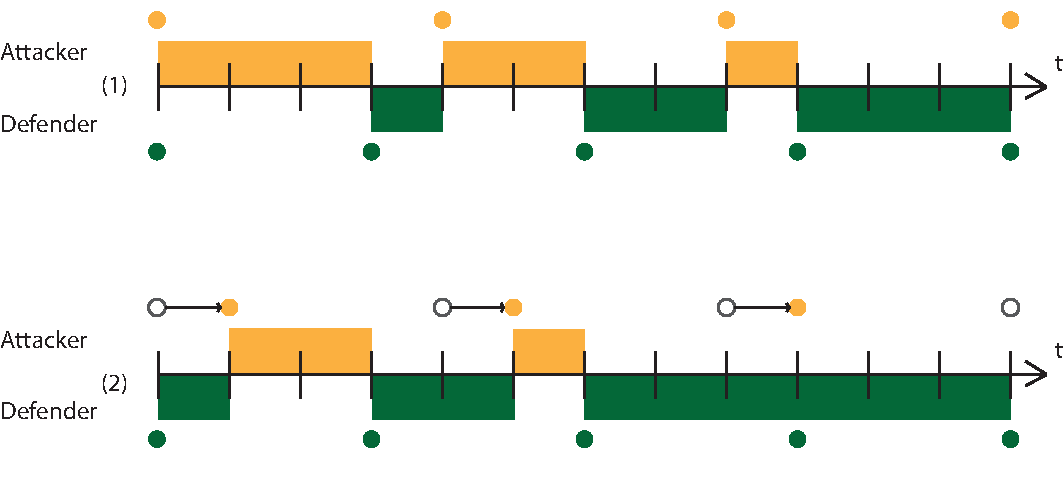
\includegraphics[scale=0.7]{../../doc/template/Images/DiffDelayCase1.pdf}
\caption{Case 1: Difference between a basic FlipIt game and a FlipIt game with a delay. Case (1) is the FlipIt game without a propagation delay and case (2) is with a propagation delay. The delay is denoted with an arrow. The attacker is only in control when the circle becomes orange (light grey).}
\label{fig:delaycase1}
\end{figure}




However, because of the delay required for virus propagation, the maximal time of control is reduced to $\delta_{D}-d$ , see figure \ref{fig:delaycase1}. While the probability that the attacker will move in the interval of the defender is still \textit{r}, the gain will not be half of the interval. Indeed, if the attacker plays after $\delta_{D}-d$, given the delay \textit{d}, he will never gain control in that interval (see figure \ref{tijdens interval}). 
\begin{figure}[hbtp]
\centering
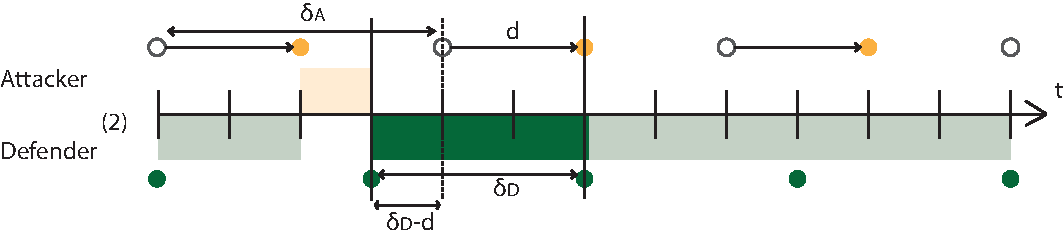
\includegraphics[scale=0.7]{../../doc/template/Images/delaydtijdens.pdf}
\caption{Attacker playing to late. If the attacker enters the defender's interval after $\delta_{D} -d$, he can not get in control in that interval.}
\label{tijdens interval}
\end{figure}The probability that the attacker plays early enough is $\dfrac{\delta_{D}-d}{\delta_{D}}$, giving the attacker an average gain of $\dfrac{\delta_{D}-d}{2}$ (the average remainder of the defender interval after the attacker flipped). If the attacker moves after the period of $\delta_{D}-d$, the gain of the attacker will be zero. The probability that this happens is  $\dfrac{d}{\delta_{D}}$. Looking at one interval of the defender, the average gain rate of the attacker can thus be expressed as follows:


\begin{equation*}
\gamma_{A}(\delta_{D},\delta_{A}) = \dfrac {1}{\delta_{D}} [ \dfrac{\delta_{D}}{\delta_{A}} \cdot \big[ \dfrac{\delta_{D}-d}{\delta_{D}} \cdot \dfrac{\delta_{D}-d}{2} + \dfrac{d}{\delta_{D}} \cdot 0 \big] ]
\end{equation*}
As the formula above is valid for each defender interval, the average gain rate over the entire game is:
\begin{equation*}
\gamma_{A}(\delta_{D},\delta_{A}) = \dfrac{(\delta_{D} -d)^{2}}{2\delta_{D}\delta_{A}}
\end{equation*}

To find the benefit, the cost of moving is subtracted from the average gain. 
\begin{equation*}
\beta_{A}(\delta_{D},\delta_{A}) = \dfrac { (\delta_{D}-d) ^{2}} {2 \delta_{D}  \delta_{A}} - \dfrac{k_{A}}{\delta_{A}}
\end{equation*}

 
 The benefit of the defender is then as follows:
\begin{equation*}
\beta_{D}(\delta_{D},\delta_{A}) = 1 - \dfrac { (\delta_{D}-d) ^{2}} {2 \cdot \delta_{D}  \delta_{A}} - \dfrac{k_{D}}{ \delta_{D}}
\end{equation*}
~~\\
For this case where $d$=0, we this equals the formula of the original FlipIt game \citep{FlipIt} [p675].\\





\subsection*{\textbf{Case 2:} $\delta_{A} \leq \delta_{D} $ (The attacker plays at least as fast as the defender.) }

First let $r = \dfrac{\delta_{D}}{ \delta_{A} }$. The intervals between two consecutive attacker's moves have length $\delta_{A}$. Consider a given attackers move interval. The probability over the attacker's phase selection that the defender moves in this interval is $\dfrac{\delta_{A}}{ \delta_{D} } = (1/r)$. Given that the defender moves within the interval of the attacker, he moves exactly once within this interval (since $\delta_{A} \leq \delta_{D} $) and his move is distributed uniformly at random. \\

A similar analysis as in case 1 for a FlipIt game without a propagation delay yields the following benefits:

\begin{equation*}
\beta_{D}(\delta_{D},\delta_{A}) = \dfrac {1} {2r} - k_{D} \alpha_{D} = \dfrac {\delta_{A}} {2\delta_{D}} - \dfrac{k_{D} }{\delta_{D}} 
\end{equation*}
\begin{equation*}
\beta_{A}(\delta_{D},\delta_{A}) =1 - \dfrac {1} {2r} - k_{A} \alpha_{A} = 1- \dfrac {\delta_{A}} {2\delta_{D}} - \dfrac{k_{A}}{ \delta_{A}}  
\end{equation*}\\

An intuitive solution for the case with a virus would be to subtract the benefit of the attacker received in each interval with the delay similarly as in case 1. This would yield the following formula:
\begin{equation*}
\beta_{A}(\delta_{D},\delta_{A})=\dfrac{(\delta_{A} - d)^2}{2\delta_{A}\delta_{D}} - \dfrac{k_{D}}{\delta_{A}}
\end{equation*}

This however results in an overestimation. 
%By simulation the game, it can be notices that the closer $\delta_{A}/\delta_{D}$ is equal to one, the better the approximation. If $\delta_{A}/\delta_{D} = 1$ the result is correct. 
The reason this formula overestimates the benefit of the attacker is that it assumes that the defender is always in control during the delay. However, if the attacker was in control in the previous interval, then he continuous to be in control during the period of the delay, see figure \ref{fig:case2}. This means that the average benefit formulas for this case cannot be derived from one interval only; what happens in the previous interval must be taken into account. \\

We know that the defender's moves are instantaneous. Therefore, it is easier to calculate the benefit of the defender. Because the defender moves slower than the attacker we know that if the defender moves during the interval of the attacker, he only moves once within this interval.

The defender will move during the interval of the attacker with a probability of $\dfrac{\delta_{A}}{\delta_{D}} $. If this happens, the defender will be in control for the remainder of this interval. In the next interval the attacker will have to regain control, meaning that during the delay, the defender stays in control, see figure \ref{fig:case2} cases (1) to (4). The defender will keep the control over the resource in the next interval over a period of the delay, namely \textit{d}. \\

Consider a timespan $\delta_{A} + d$, representing the attacker's interval followed by the delay period in his next interval. If we assume that $\delta_{A}+d<\delta_{D}$, we can infer that the defender will never move twice during this timespan.
Because $d + \delta_{A} \leq \delta_{D}$ the next move of the defender in this second interval will never occur during the delay, meaning that the entire delay can be considered as an extra benefit resulting of a play in the previous interval. 
So, every time the defender plays, he will get an average gain of $\dfrac{\delta_{A}}{2}$ in the interval where he plays and in the next interval will always receive a extra gain of $d$, yielding a total average gain per interval of
$\dfrac{(d+\dfrac{\delta_{A}}{2})}{\delta_{A}}$

For the case with a delay we consider two cases, Case a and Case b, depending on whether the delay is shorter or longer than the difference between the attacker's and the defender's period.  \\

\begin{figure}[hbtp]
\centering
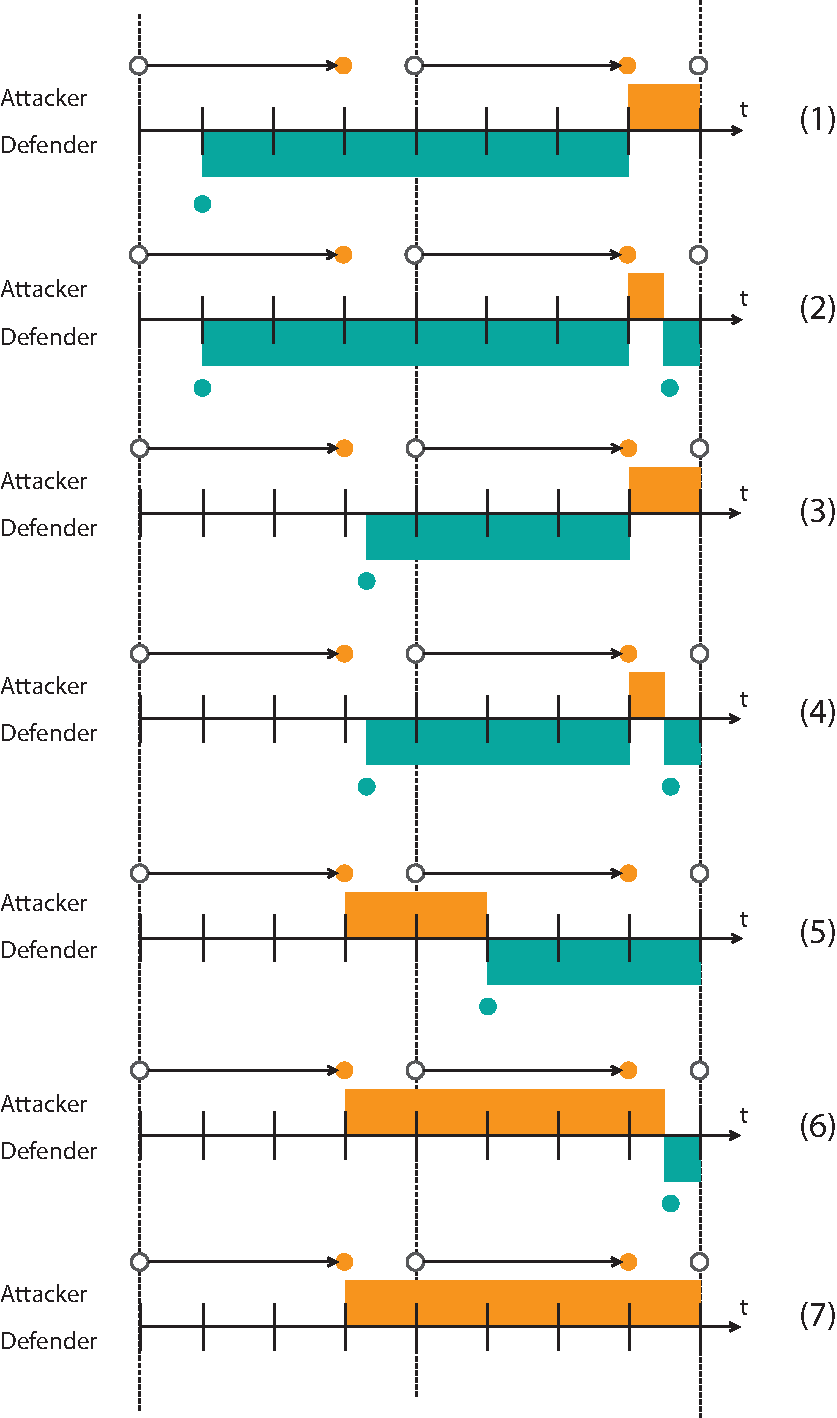
\includegraphics[scale=0.7]{../../doc/template/Images/FlipIt2.pdf}
\caption{All possible cases for the attacker and the defender in Case 2.A where $d + \delta_{A} < \delta_{D}$. As can be seen in cases (1) to (4), the defender will have control during a period of \textit{d} over the resource in the next interval when the defender has flipped in the previous interval.}
\label{fig:case2}
\end{figure}

\subsubsection*{\textbf{Case a:} $d + \delta_{A} \leq \delta_{D}$}
%The first case is where the defender's period is larger than the sum of the delay and the attacker's period. 
In this case the delay will never be counted twice in the defender's  benefit formula. To determine the total gain rate of the defender we need to know the probability that the defender will move during an interval and what the average time is that the defender controls the resource. Given that if the defender moves he will always benefit entirely from a period of delay in the next interval of the attacker, his total gain is $\dfrac{(d+\dfrac{\delta_{A}}{2})}{\delta_{A}}$ \todo{formule valt uit de lucht} in one interval. The total gain  rate of the defender is then the probability that the defender will move during an interval of the attacker multiplied by the total average gain per interval: 

\begin{equation*}\label{first}
\gamma_{D}(\delta_{D},\delta_{A}) = \dfrac{\delta_{A}}{\delta_{D}} \cdot \dfrac{(d+\dfrac{\delta_{A}}{2})}{\delta_{A}} 
\end{equation*}
\begin{equation*}\label{first}
\gamma_{D}(\delta_{D},\delta_{A}) = \dfrac{\delta_{A}}{2\delta_{D}} + \dfrac{d}{\delta_{D}} 
\end{equation*}\\
This yields the following benefit formula:
\begin{equation*}\label{first}
\beta_{D}(\delta_{D},\delta_{A}) = \dfrac{\delta_{A}}{2\delta_{D}} + \dfrac{d}{\delta_{D}} - \dfrac{k_{D}}{ \delta_{D}}
\end{equation*}\\

The benefit for the attacker will be as follows:
\begin{equation*}\label{first}
\beta_{A}(\delta_{D},\delta_{A}) = 1 -\dfrac{\delta_{A}}{2\delta_{D}} - \dfrac{d}{\delta_{D}} - \dfrac{k_{A}}{ \delta_{A}}
\end{equation*}\\



It is crucial that $ \delta_{D}$ is at least as large as $d + \delta_{A}$. If not, the defender can move during the delay in the interval following the interval in which the defender already moved. This would result in an overlap between the average gain of $\dfrac{\delta_{A}}{2} +d$ and the delay. The above benefit formula would then include to much gain for the defender: the potential overlap during the delay would be counted twice. See figure \ref{countedtwice}\\

\begin{figure}[hbtp]
\centering
\caption{Cases where the delay would be counted twice.}
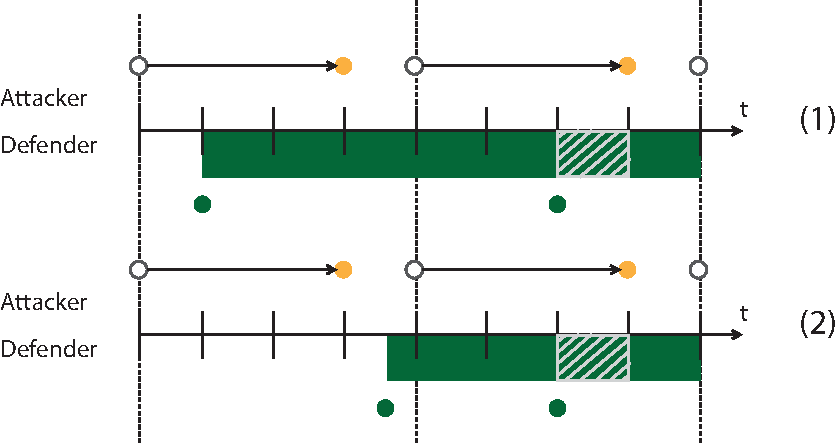
\includegraphics[scale=0.7]{Images/flipcase2nb.pdf}
\label{countedtwice}
\end{figure}

~~ \\
\subsubsection*{\textbf{Case b:} $d + \delta_{A} \geq \delta_{D}$}
~~~\\

To obtain the formula in case of a too long delay, we therefore need to subtract this overlapping gain from the above formula. 
Since $\delta_{D} \geq \delta_{A}$, if the defender enters the interval immediately after the attacker has played, the defender cannot have played in the previous interval. In that case, there is no overlap. So the problem of the overlap only appears if the defenders enters late enough and thus only the last part of the delay is subject to overlap. The larger the difference between the interval of the defender and the attacker, the smaller the risk of overlap. Concretely, only the last part of length $d - (\delta_{D} - \delta_{A})$ is subject to overlap. Hence, the probability of overlap is $\dfrac{ d - (\delta_{D} - \delta_{A})}{\delta_{D}}$ and the average gain will be half of this interval:  $\dfrac{ d - (\delta_{D} - \delta_{A})}{2}$.  The gain rate to be subtracted is therefore:\\

\begin{equation*}
\dfrac{1} {\delta_{A}} \cdot \dfrac{d - (\delta_{D} - \delta_{A})}{\delta_{D}} \cdot \dfrac{d - (\delta_{D} - \delta_{A})}{2}
\end{equation*}

The total gain rate for the defender is obtained by subtracting this term from the gain rate of case a:
 \begin{equation*}
\gamma_{D}(\delta_{D},\delta_{A}) = \dfrac{\delta_{A}}{\delta_{D}} \cdot \dfrac{(d+\dfrac{\delta_{A}}{2})}{\delta_{A}} - \dfrac{(d - (\delta_{D} - \delta_{A}))^{2}}{2 \delta_{D} \delta_{A}}
\end{equation*}
\begin{equation*}
\gamma_{D}(\delta_{D},\delta_{A}) = \dfrac{\delta_{A}}{2\delta_{D}} + \dfrac{d}{\delta_{D}} - \dfrac{(d - (\delta_{D} - \delta_{A}))^{2}}{2 \delta_{D} \delta_{A}}
\end{equation*}\\
This yields in the following benefit formula:
\begin{equation*}
\beta_{D}(\delta_{D},\delta_{A}) = \dfrac{\delta_{A}}{2\delta_{D}} + \dfrac{d}{\delta_{D}} - \dfrac{k_{D}}{ \delta_{D}} - \dfrac{(d - (\delta_{D} - \delta_{A}))^{2}}{2 \delta_{D} \delta_{A}}
\end{equation*}\\
 
Consequently, the benefit for the attacker will be:
\begin{equation*}
\beta_{A}(\delta_{D},\delta_{A}) = 1 -\dfrac{\delta_{A}}{2\delta_{D}} - \dfrac{d}{\delta_{D}} - \dfrac{k_{A}}{ \delta_{A}} + \dfrac{(d - (\delta_{D} - \delta_{A}))^{2}}{2 \delta_{D} \delta_{A}}
\end{equation*}\\

%~~\\
%\subsection{Conclusion of this chapter}
%\begin{description}
%\item[-]
%\item[-]
%\item[-]
%\end{description}